%\documentclass[preprint,authoryear,review,12pt]{elsarticle}
\documentclass{frontiersSCNS}

%% Use the option review to obtain double line spacing
%% \documentclass[preprint,review,12pt]{elsarticle}

%% Use the options 1p,two column; 3p; 3p,twocolumn; 5p; or 5p,twocolumn
%% for a journal layout:
%% \documentclass[final,1p,times]{elsarticle}
%% \documentclass[final,1p,times,twocolumn]{elsarticle}
%% \documentclass[final,3p,times]{elsarticle}
%% \documentclass[final,3p,times,twocolumn]{elsarticle}
%% \documentclass[final,5p,times]{elsarticle}
%% \documentclass[final,5p,times,twocolumn]{elsarticle}


\usepackage{color}
\usepackage{multirow,booktabs,ctable,array}
\usepackage{lscape}
\usepackage{amsmath}
\usepackage{lineno}
\usepackage{ulem}
\usepackage{setspace}
\usepackage{listings}
\usepackage{float}

\usepackage{algorithm}
\usepackage{algpseudocode}

\floatstyle{plain}
\newfloat{command}{thp}{lop}
\floatname{command}{Command}

%\usepackage[nomarkers,notablist]{endfloat}

%% if you use PostScript figures in your article
%% use the graphics package for simple commands
%% \usepackage{graphics}
%% or use the graphicx package for more complicated commands
%% \usepackage{graphicx}
%% or use the epsfig package if you prefer to use the old commands
%% \usepackage{epsfig}

%% The amssymb package provides various useful mathematical symbols
\usepackage{amssymb}
%% The amsthm package provides extended theorem environments
% \usepackage{amsthm}

 \usepackage{makecell}

%% The lineno packages adds line numbers. Start line numbering with
%% \begin{linenumbers}, end it with \end{linenumbers}. Or switch it on
%% for the whole article with \linenumbers after \end{frontmatter}.
%% \usepackage{lineno}

%% natbib.sty is loaded by default. However, natbib options can be
%% provided with \biboptions{...} command. Following options are
%% valid:

%%   round  -  round parentheses are used (default)
%%   square -  square brackets are used   [option]
%%   curly  -  curly braces are used      {option}
%%   angle  -  angle brackets are used    <option>
%%   semicolon  -  multiple citations separated by semi-colon
%%   colon  - same as semicolon, an earlier confusion
%%   comma  -  separated by comma
%%   numbers-  selects numerical citations
%%   super  -  numerical citations as superscripts
%%   sort   -  sorts multiple citations according to order in ref. list
%%   sort&compress   -  like sort, but also compresses numerical citations
%%   compress - compresses without sorting
%%
%% \biboptions{comma,round}

% \biboptions{}

\providecommand{\OO}[1]{\operatorname{O}\bigl(#1\bigr)}

\graphicspath{{./Figures/}
              {./Results/}}

\long\def\symbolfootnote[#1]#2{\begingroup%
\def\thefootnote{\fnsymbol{footnote}}\footnote[#1]{#2}\endgroup}

    \usepackage{color}

    \definecolor{listcomment}{rgb}{0.0,0.5,0.0}
    \definecolor{listkeyword}{rgb}{0.0,0.0,0.5}
    \definecolor{listnumbers}{gray}{0.65}
    \definecolor{listlightgray}{gray}{0.955}
    \definecolor{listwhite}{gray}{1.0}

\newcommand{\lstsetcpp}
{
\lstset{frame = tb,
        framerule = 0.25pt,
        float,
        fontadjust,
        backgroundcolor={\color{listlightgray}},
        basicstyle = {\ttfamily\scriptsize},
        keywordstyle = {\ttfamily\color{listkeyword}\textbf},
        identifierstyle = {\ttfamily},
        commentstyle = {\ttfamily\color{listcomment}\textit},
        stringstyle = {\ttfamily},
        showstringspaces = false,
        showtabs = false,
        numbers = none,
        numbersep = 6pt,
        numberstyle={\ttfamily\color{listnumbers}},
        tabsize = 2,
        language=[ANSI]C++,
        floatplacement=!h,
        caption={},
        captionpos=b,
        }
}


\copyrightyear{}
\pubyear{}

\def\journal{Neuroscience}%%% write here for which journal %%%
\def\DOI{}
\def\articleType{Methods}
\def\keyFont{\fontsize{8}{11}\helveticabold }
%\def\firstAuthorLast{Tustison {et~al.}} %use et al only if is more than 1 author
\def\firstAuthorLast{Tustison and Avants} %use et al only if is more than 1 author
\def\Authors{Nicholas J. Tustison\,$^{1,*}$ and Brian B. Avants\,$^{2}$
 }
% Affiliations should be keyed to the author's name with superscript numbers and be listed as follows: Laboratory, Institute, Department, Organization, City, State abbreviation (USA, Canada, Australia), and Country (without detailed address information such as city zip codes or street names).
% If one of the authors has a change of address, list the new address below the correspondence details using a superscript symbol and use the same symbol to indicate the author in the author list.
\def\Address{$^{1}$University of Virginia, Department of Radiology and Medical Imaging, Charlottesville, VA, USA \\
$^{2}$Penn Image Computing and Science Laboratory, University of Pennsylvania, Department of Radiology, Philadelphia, PA, USA }
% The Corresponding Author should be marked with an asterisk
% Provide the exact contact address (this time including street name and city zip code) and email of the corresponding author
\def\corrAuthor{Nick Tustison}
\def\corrAddress{University of Virginia, Department of Radiology and Medical Imaging,  480 Ray C Hunt Drive, Charlottesville, VA, 22903}
\def\corrEmail{ntustison@virginia.edu}

% \color{FrontiersColor} Is the color used in the Journal name, in the title, and the names of the sections


\begin{document}
\onecolumn
\firstpage{1}

\title[Explicit B-spline regularization]{Explicit B-spline regularization in diffeomorphic image registration}
\author[\firstAuthorLast ]{\Authors}
\address{}
\correspondance{}
\editor{}
\topic{}

\maketitle

%\linenumbers


\begin{abstract}
Important methodological developments in the evolution of image registration algorithms include those
in which the correspondence relationship is characterized by diffeomorphisms.
The  popularity of these approaches is due largely to their
topological properties and success in providing biologically plausible
solutions to small and large deformation
estimation problems. Popular variants of diffeomorphic algorithms include those characterized by
time-varying and constant velocity fields, and symmetrical considerations.
Prior information (i.e. regularization) is used to enforce transform plausibility taking the form of physics-based constraints or through some approximation thereof, e.g. Gaussian smoothing of the vector fields (a la Thirion's Demons \citep{thirion1998}).  In the context of the original Demons' framework, the traditional free-form deformation method can be viewed as a variant in which explicit regularization is achieved through the B-spline basis functions.
This characterization can be used to provide alternative B-spline ``flavored'' diffeomorphic image registration solutions with several advantages which we describe in this work.  Implementation is open source and available through the Insight Toolkit and our Advanced Normalization Tools (ANTs) repository.  A thorough comparative evaluation with the well-known SyN algorithm \citep{avants2008}, implemented within the same framework, and its B-spline analog is performed using open data and open source evaluation tools.
\tiny
\keyFont{ \section{Keywords:}
open science, best practices, reproducibility, software }
\end{abstract}







%\begin{itemize}
%  \item We should trace the use of explicit regularization from
%  \item The advantage is not the parameterization per se (contra Tom) but the other
%  benefits listed (Vercuraten, Non-parametric Diffeomorphic Image Registration with the Demons Algorithm).
%  \item This paper provides the link between traditional B-spline approaches and other
%  approaches, i.e. Gaussian smoothing, Demons,
%  \item The ability to weight the boundaries provides a natural way of enforcing Dirichlet boundary conditions which is consistent with the geometric (i.e. B-spline) modeling. (Cahill, SPIE 2012).
%  \item Fluid vs. Elastic B-spline registration algorithms
%  \item Fitting a continuous object (as opposed to the discrete gaussian which has no
%        continuity nor does convolution using FFT provide continuity constraints).
%  \item Fitting routine is parallelized for fast sampling as is sampling to go from continuous object to sampled b-spline object.
%  \item Everything is open-source in ANTs and ITK.
%  \item Also, we should talk about how B-spline SyN works really well for large smoothing  but Gaussian SyN does not.
%\end{itemize}
%
%
%Also talk about fixed boundary conditions in the context of Nathan Cahill, SPIE 2012.
%




%% MSC codes here, in the form: \MSC code \sep code
%% or \MSC[2008] code \sep code (2000 is the default)

%%
%% Start line numbering here if you want
%%
% \linenumbers

%% main text

\section{Introduction}
%State the objectives of the work and provide an adequate background, avoiding a detailed literature survey or a summary of the results.

Establishment of anatomical and functional correspondence
is a crucial step towards gaining insight into certain biological
sciences.  Neuroscience research efforts, such as characterizing
brain morphology, require accurate and robust methods for
producing such mappings.  The
extensive literature detailing methodology is evidence of the rich history of
algorithmic development which continues contemporaneously.
We highlight several key contributions which are particularly relevant to the work presented.

Free-form deformation (FFD) image registration, characterized by  regularization based on the B-spline basis functions, has several
advantages including algorithmic simplicity,
good performance, desirable properties, and several available
implementations.  Current research was
preceded by related work for
geometric modeling \citep{sederberg1986} and originated with such important
contributions as \cite{szeliski1997,thevenaz1998,rueckert1999}.
Continued development within this early spline-based paradigm produced additional innovations such as integrated similarity metrics \citep[e.g.][]{mattes2003}, additional transformation constraints \citep[e.g.][]{rohlfing2003}, and notable open source implementations \citep[e.g.][]{ibanez2005,klein2010,shackleford2010}.

Parallel to this branch of algorithmic progress are the informally
denoted ``dense transforms''
perhaps best exemplified by Thirion's seminal contribution \citep{thirion1998}.
Relationships with earlier elastic \citep{bajcsy1989,gee1993} and fluid \citep{christensen1996} registration methods are detailed in
the works of \cite{bro-nielsen1996} and \cite{pennec1999} who observe that
smoothing via Gaussian convolution, a defining characteristic of Demons,
of the update or displacement
field is a greedy approximation for solving the partial differential equations governing
the physics of an elastic or fluid deformation, respectively.  However, the use of such
approximations entails that physical properties, such as topological
regularity, are no longer guaranteed.

It is interesting to note that within this context, traditional FFD algorithms
can be viewed as a type of fluid-like Demons approach
where, rather than projecting the update field to the space
of regularized fields using Gaussian convolution, gradient fields
are projected to a smooth space characterized by the B-spline
basis functions.  This analogy was hinted at in our earlier work \citep{tustison2009} where we showed that fitting the update field to a B-spline object using a fast approximation routine \citep{tustison2006} is equivalent to a preconditioning of the standard gradient used in gradient descent-based FFD optimization.
This preconditioning is used to mitigate the hemstitching effect induced by the ill-conditioned nature of the traditional gradient-based FFD formulation.
Further details can be gleaned from the ITK implementation of this
earlier work%
\footnote{
http://www.itk.org/Doxygen/html/classitk\_1\_1BSplineSmoothingOnUpdateDisplacementFieldTransform.html
}
which permits both B-spline smoothing on the update (``viscous'') and total (``elastic'')
displacement fields at each iteration (cf
analogous Gaussian, i.e. Demons, implementation%
\footnote{
http://www.itk.org/Doxygen/html/classitk\_1\_1GaussianSmoothingOnUpdateDisplacementFieldTransform.html
}).

Continuing from the work of \cite{christensen1996} and subsequent exploration into the mathematical formalisms of diffeomorphisms \citep[e.g.][]{dupuis1998},
the well-known Large Deformation Diffeomorphic Metric Mapping (LDDMM) algorithm
was proposed in \cite{beg2005}.  In contrast to the mapping produced
by \cite{christensen1996}, LDDMM yields the geodesic solution in the space of diffeomorphisms between two images. Since its introduction, LDDMM has
inspired much innovation in the image registration literature.  Applying
the log-Euclidean framework of \cite{arsigny2006}, DARTEL (Diffeomorphic Anatomic Registration using Exponential Lie algebra) uses a constant velocity field parameterization to provide a fast, diffeomorphic alternative \citep{ashburner2007}. Additionally, symmetrical considerations in the velocity field parameterization are discussed in \cite{avants2008} in the context of a cross correlation similarity metric which minimizes the bias of the resulting transformation when selecting the ``fixed'' and ``moving'' images.  A greedy version of this algorithm has proven successful in neuroimaging \citep{klein2009} and pulmonary \citep{murphy2011} applications.



%Other important image registration research
%reflected increased emphasis on topological transformation considerations
%in modeling biological/physical systems where topology is
%consistent throughout the course of deformation or a
%homeomorphic relationship is assumed between image domains.
%Methods such as LDDMM \citep{beg2005} optimize time-varying velocity field
%flows to yield diffeomorphic transformations.


Although many extensions of LDDMM rely
on some form of Gaussian convolution for
regularization \citep[e.g.][]{risser2011}, there has been significant interest in constraining
FFD approaches to the space of diffeomorphisms.
An early attempt reported in \cite{rueckert2006} enforced
diffeomorphic transforms
by concatenating multiple FFD transforms, each of which is constrained
to describe a one-to-one mapping.
\cite{modat2011} incorporated the log-Euclidean
framework for enforcing diffeomorphic transformations and ensuring invertibility.  Similarly, the work of \cite{de-craene2011} provided
a full LDDMM-style algorithm based on B-splines called
{\em temporal free-form deformation} in which the
time-varying velocity field
is modeled using a 4-D B-spline object (3-D + time).  Numerical integration of the mapping propagated within the velocity field yields the transform between parameterized time points.

As alluded to earlier, B-spline approximation can also be used
for regularizing vector fields in an analogous fashion as
Gaussian convolution.  In this vein and similar to
\cite{de-craene2011}, we reported in \cite{tustison2012a,tustison2012}
the use of an $n$-D + time B-spline object to
represent the characteristic velocity fields.  However, we use the
directly manipulated free-form deformation formulation to improve the solution convergence and actual results.  This also facilitates modeling
temporal periodicity and the enforcement of stationary boundaries.

Both this latter work \citep{tustison2012a} and our earlier work
\citep{tustison2009} demonstrate that our DMFFD framework is potentially
applicable to the
entire gamut of diffeomorphic registration algorithms and provides
unique ``flavors'' of smoothing possibilities.  However, differences
between the two approaches produce characteristically different
solutions.  In addition to
smoothing kernel differences, Gaussian
convolution tends to ``flatten'' the signal in contrast to an
approximation or fitting of the signal provided by the DMFFD
approach.  Also, whereas
convolution operates entirely within the discrete space,
the fitting process constructs a continuous object prior
to any discrete sampling.  Further elaboration on these differences
are discussed in subsequent sections.

Variants of three popular diffeomorphic algorithms and their DMFFD analogs
(LDDMM%
\footnote{
\begin{itemize}
\item http://www.itk.org/Doxygen/html/classitk\_1\_1TimeVaryingVelocityFieldTransform.html
\item http://www.itk.org/Doxygen/html/classitk\_1\_1TimeVaryingBSplineVelocityFieldTransform.html
\end{itemize}
},
DARTEL%
\footnote{
\begin{itemize}
\item http://www.itk.org/Doxygen/html/classitk\_1\_1GaussianExponentialDiffeomorphicTransform.html
\item http://www.itk.org/Doxygen/html/classitk\_1\_1BSplineExponentialDiffeomorphicTransform.html
\end{itemize}
},
 and SyN%
\footnote{
\begin{itemize}
\item http://www.itk.org/Doxygen/html/classitk\_1\_1SyNImageRegistrationMethod.html
\item http://www.itk.org/Doxygen/html/classitk\_1\_1BSplineSyNImageRegistrationMethod.html
\end{itemize}
})
were implemented by the authors
as part of the recent refactoring of the open source
Insight Toolkit (ITK) although related work had been
previously implemented within the popular Advanced
Normalization Tools (ANTs).%
\footnote{
http://stnava.github.io/ANTs
}
Given the popularity and excellent performance of the symmetric normalization (SyN) algorithm, our focus in this work is
its B-spline equivalent which we denote as ``B-spline SyN.''
Evaluation and comparisons of the respective algorithmic instantiations
are performed using the \verb#antsRegistration# program found
in the ANTs repository (also originally developed by the authors \citep{tustison2012}).  This permits a direct algorithmic comparison
as potential sources for implementation bias have been removed \citep{tustison2013}.  Additionally, in the spirit of open science,
all text, figures, and
scripts to reproduce the results contained in this work are publicly available online.%
\footnote{
https://github.com/ntustison/BSplineMorphisms
}

\section{Material and Methods}

\subsection{Theoretical Overview}

Given the spatial domain $\Omega$ of $d-$dimensionality
defined over image $I$, a diffeomorphic
mapping, $\phi$, parameterized over $t \in [0,1]$ transforms the image
$I$ to the target image $J$ using $I\circ\phi(\mathbf{x},1)$ where the
geodesic path $\phi(\mathbf{x},t)$ is described by \citep{beg2005}
\begin{align}
  \inf_{\phi} \left( \int_0^1 \|v(t)\|_L^2 dt +
                     \int_{\Omega} | I \circ \phi^{-1}(\mathbf{x},1) - J |^2 d\Omega
              \right).
  \label{eq:lddmm}
\end{align}
$\phi$ is generated as the solution of the ordinary differential equation
\begin{align}
  \frac{d \phi(\mathbf{x},t)}{dt} = v( \phi(\mathbf{x},t), t ),\,\, \phi(\mathbf{x},0) = \mathbf{Id}
\label{eq:ode}
\end{align}
where $v$ is a time-dependent smooth field (as dictated by the functional norm $L$), $v : \Omega \times t
\rightarrow \mathrm{R}^d$ parameterized by $t \in [0,1]$.  Diffeomorphic mappings
between parameterized time points $\{t_a,t_b\} \in [0,1]$
are obtained from  Eq. (\ref{eq:ode}) through integration of the transport
equation, viz.
\begin{align}
  \label{eq:integral}
\phi(\mathbf{x},t_b) &= \phi(\mathbf{x},t_a) + \int_{t_a}^{t_b} v(\phi(\mathbf{x}), t) dt.
\end{align}
%and $L$ is the functional norm which enforces velocity field regularity.

However,
as pointed out in \cite{avants2008}, implementations of this standard
LDDMM formulation are negatively affected by the lack of optimization
symmetry where arbitrary assignment of fixed and moving images could
lead to different solutions despite the fact that the theoretical
geodesic solution describes the same path forwards and backwards.
This observation led to the symmetric
formulation of Eq. (\ref{eq:lddmm}) found in \cite{avants2008}:
\begin{align}
  \inf_{\phi_1} \inf_{\phi_2} \left(
                     \int_0^{0.5} \left( \|v_1(t)\|_L^2 + \|v_2(1-t)\|_L^2 \right) dt +
                     \int_{\Omega} | I \circ \phi_1^{-1}(\mathbf{x},0.5)
                           - J \circ \phi_2^{-1}(\mathbf{x},0.5) |^2 d\Omega
              \right)
\end{align}
where
\begin{align}
  \frac{d \phi_i(\mathbf{x},t)}{dt} = v_i( \phi_i(\mathbf{x},t), t ),\,\, \phi_i(\mathbf{x},0) = \mathbf{Id}, \,\, i \in \{1,2\}
\end{align}
with extension to arbitrary similarity metric choice, i.e. the second
term is replaced with
\begin{align}
\int_{\Omega} \Pi_{\sim}
                          \left( I \circ \phi_1^{-1}(\mathbf{x},0.5),
                           J \circ \phi_2^{-1}(\mathbf{x},0.5) \right) d\Omega
\end{align}
with a popular choice for $\Pi_{\sim}$ being a local neighborhood cross
correlation \citep{avants2008,avants2011}.
Note that
$t$ is parameterized in opposite directions between $\phi_1$ and $\phi_2$.
A diagrammatic
illustration of the explicit symmetry associated with SyN is shown in
Figure \ref{fig:syn}.

\begin{figure}[htb]
  \centering
  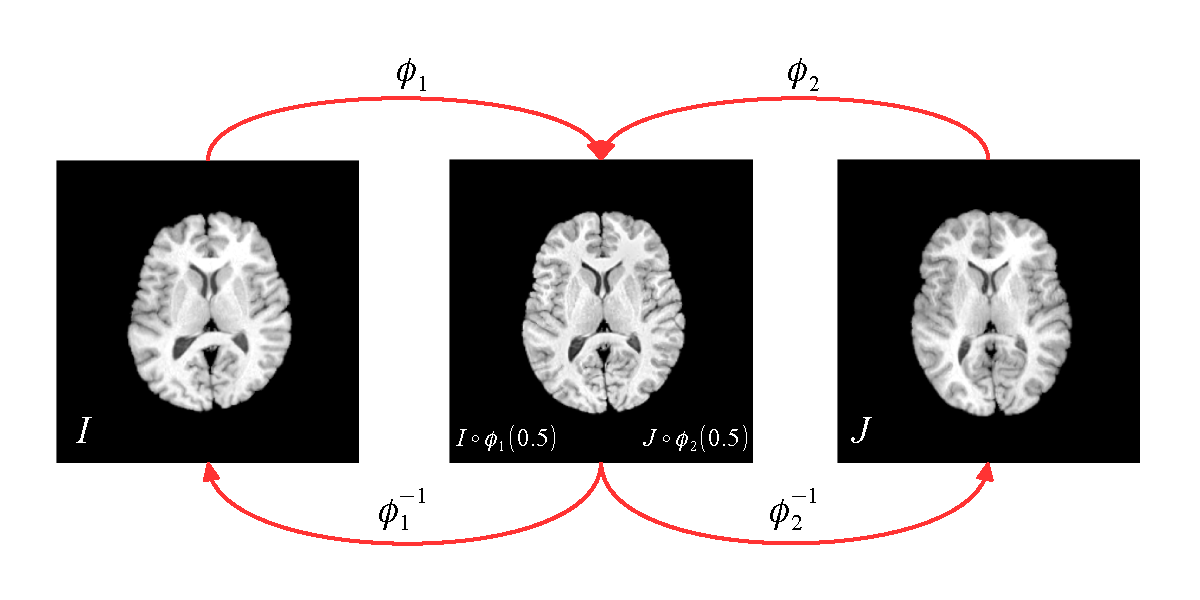
\includegraphics[width=0.95\textwidth]{SyN.pdf}
  \caption{Illustration of the greedy SyN formulation.  Given images
  $I_A$ and $I_B$, the symmetric set-up requires finding the two
  transform pairs $\left(\phi_1,\phi_1^{-1}\right)$
  $\left(\phi_2,\phi_2^{-1}\right)$ which map to/from
  the respective images to the midway point. During
  optimization, the update field at each iteration is
  determined from the metric field gradient taken at
  the midway point, i.e.
  $\nabla \Pi_{\sim} \left(I\circ\phi_1(0.5),J\circ\phi_2(0.5)\right)$.
  The full
  forward and inverse transforms are found through
  composition, i.e. $\phi=\phi_1 \circ \phi_2^{-1}$ and
  $\phi^{-1}=\phi_2 \circ \phi_1^{-1}$.
  }
  \label{fig:syn}
\end{figure}

\subsubsection{St. Nava's Theory of Greed and Original SyN}

Although presenting a rigorous framework for image registration solutions
with desirable properties, the complexity of these diffeomorphic methodologies
requires substantial computational resources.  For typical 3-D neuroimaging
applications, the corresponding solutions require numerical integration over
and storage of 4-D velocity fields at each iteration which is limiting for
many common, contemporary processing infrastructures.

Therefore, in addition to the full-scale
symmetric SyN offering described in \cite{avants2008}, the authors therein
provided a ``greedy'' alternative which has demonstrated superior performance
in various applications \citep{avants2011,klein2009,murphy2011}%
\footnote{
SyN was also the standard registration for the MICCAI 2013
Workshop on Segmentation:  Algorithms Theory, and Applications (SATA)
and corresponding challenge (https://masi.vuse.vanderbilt.edu/workshop2013).
}
while simultaneously being capable of running with limited computational
resources.  In this variant, the discrete time-parameterized
velocity field samples are restricted to their respective
endpoints, i.e. the $v_i(\mathbf{x},t)$ are sampled at $t \in \{0,0.5,1\}$
implying simultaneous storage of only four transform vector fields
$\phi_1(\mathbf{x})$,
$\phi_1^{-1}(\mathbf{x})$, $\phi_2(\mathbf{x})$, and $\phi_2^{-1}(\mathbf{x})$
(cf Figure \ref{fig:syn}).  The algorithmic steps are briefly sketched
in Algorithm \ref{alg:syn}.

\begin{algorithm}
\caption{SyN algorithmic overview}
\label{alg:syn}
\begin{algorithmic}
\State $\phi_i \leftarrow \mathbf{Id}$, $\phi_i^{-1} \leftarrow \mathbf{Id}$
\Comment $i \in \{1,2\}$
\State $n \leftarrow 1$
\While {not converged}
  \State $v_1^n \leftarrow \nabla \Pi_{\sim} \left(I\circ\phi_1^{n-1},J\circ\phi_2^{n-1}\right)$
  \State $v_2^n \leftarrow \nabla \Pi_{\sim} \left(J\circ\phi_2^{n-1},I\circ\phi_1^{n-1}\right)$
  \State $v_i^n \leftarrow S_v( v_i^n )$      \Comment $S_v$ is a smoothing operation on the update transform field
  \State $\phi_i^n \leftarrow S_\phi( v_i^n \circ \phi_i^{n-1} )$      \Comment $S_\phi$ is a smoothing operation on the total transform field
  \State $\left(\phi_i^n\right)^{-1} \leftarrow Inv\left(\phi_i^n, \left(\phi_i^{n-1}\right)^{-1}\right)$
    \Comment Inverse field estimation described in \cite{avants2008}
  \State $n \leftarrow n + 1$
\EndWhile
\State \Return $\phi \leftarrow \phi_1 \circ \phi_2^{-1}$, $\phi^{-1} \leftarrow \phi_2 \circ \phi_1^{-1}$
\end{algorithmic}
\end{algorithm}


\subsubsection{Directly Manipulated Free-Form Deformation Diffeomorphic Analogs}

Although several velocity field regularization
operators have been proposed, many algorithmic instantiations
default to Gaussian smoothing due to its simplicity both in implementation
and complexity terms.
Extending the work presented in \cite{tustison2009,tustison2012},
the DMFFD approach is a viable and practical alternative
for explicit regularization in diffeomorphic image registration.

As we mentioned previously, it has been shown that the preconditioned
gradient of the B-spline object is equivalent to a B-spline approximation
smoothing operation on the spatial derivative of the similarity metric
gradient \citep{tustison2009}. In the case of
$d$-dimensional image registration, the time-dependent velocity field can be
represented
as a $(d + 1)$-dimensional B-spline object
\begin{align}
v(\mathbf{x}, t) = \sum_{i_1=1}^{X_1}\ldots\sum_{i_d=1}^{X_d}\sum_{i_t=1}^T v_{i_1,\ldots,i_d,i_t} B_{i_t}(t) \prod_{j=1}^d B_{i_j}(x_j)
\end{align}
where $v_{i_1,\ldots,i_d,i_t}$ is a $(d+1)$-dimensional control point lattice
characterizing the velocity field and $B(\cdot)$ are the univariate B-spline
basis functions separately modulating regularity in the solution for each parametric dimension.  The preconditioned gradient analog for updating the velocity
field is as follows \citep{tustison2012}:
$\delta v_{i_1,\ldots,i_d,i_t}$, given the similarity metric, $\Pi_\sim$,
\begin{align}
\label{eq:dmffd}
  \delta v_{i_1,\ldots,i_d,i_t} &= \left( \sum_{c=1}^{N_{\Omega} \times N_t} \left( \frac{\partial \Pi_\sim}{\partial \mathbf{x}} \right)_c B_{i_t}(t^c)\prod_{j=1}^d B_{i_j}(x_j^c)  \right. \nonumber \\
  &\cdot \left. \frac{B_{i_t}^2(t^c) \prod_{j=1}^d B_{i_j}^2 (x_j^c)}
  {\sum_{k_1=1}^{r+1}\ldots\sum_{k_d=1}^{r+1} \sum_{k_t=1}^{r+1} B_{k_t}^2(t^c)
  \prod_{j=1}^d B_{k_j}^2 (x_j^c)} \right) \nonumber \\
  &\cdot\left({\sum_{c=1}^{N_{\Omega}\times N_t}B_{i_t}^2(t^c) \prod_{j=1}^d B_{i_j}^2 (x_j^c)} \right) ^{-1}
\end{align}
which is a slight modification of Eqn. (21) in \cite{tustison2009}
which takes into account the temporal locations of the
dense gradient field sampled in $t \in [0,1]$. $N_t$ and $N_\Omega$ are the number
of time point samples and the number of voxels in the reference image domain, respectively.
$r$ is the spline order in all dimensions%
\footnote{
In terms of implementation spline orders can be specified separately for each dimension but, for simplicity,
we only specify a single spline order.
}
and $c$ indexes the spatio-temporal dense metric gradient sample.
Additionally, in \cite{tustison2006} it was shown that one could associate each
a sample, $\left( \frac{\partial \Pi}{\partial \mathbf{x}}\right)_c$ with a confidence
weighting.  Thus, in order to enforce stationary boundaries, we
assign image boundary metric gradients a value of zero with a corresponding
large confidence value.




\subsection{Implementation}

Although various methods exist for solving Eqns. (\ref{eq:ode}) and (\ref{eq:integral}),
we use $4^{th}$-order Runge-Kutta, i.e.
\begin{align}
  \phi_{n+1} &= \phi_{n} + \frac{1}{6}\left( k_1 + 2k_2 + 2k_3 + k_4 \right) \\
  t_{n+1} &= t_{n} + \Delta t \\
  \phi_0 &= \phi(t_0)
\end{align}
where
\begin{align}
  k_1 &= v\left( \phi_{n}, t_{n} \right)\Delta t \\
  k_2 &= v\left( \phi_{n} + \frac{k_1}{2}, t_{n} + \frac{\Delta t}{2} \right)\Delta t \\
  k_3 &= v\left( \phi_{n} + \frac{k_2}{2}, t_{n} + \frac{\Delta t}{2} \right)\Delta t \\
  k_4 &= v\left( \phi_{n} + k_3, t_{n} + \Delta t \right)\Delta t
\end{align}
which provides a more stable and reliable alternative than other numerical
methods \citep{press2007}.

\subsection{Evaluation Data}

We take inspiration from the well-known
Klein comparative study in which 14 image registration
algorithms were evaluated based on performance
on publicly available labeled brain data \citep{klein2009}.
Based on the final rankings, the SyN algorithm is one
of the top-performing registration algorithms.  Its relative
performance coupled with its public availability has made
it a de facto standard for algorithmic comparison.

For our evaluation, we used the same data as that in the
Klein study.  Specifically, we used the data sets denoted as:
\begin{itemize}
  \item MGH10
  \item CUMC12
  \item IBSR18
  \item LPBA40
\end{itemize}
which are available for download from Arno Klein's website.%
\footnote{
http://mindboggle.info/papers/evaluation\_NeuroImage2009.php
}
We also use the labeled brain data provided at the
MICCAI 2012 Grand Challenge and Workshop on Multi-Atlas
Labeling%
\footnote{
https://masi.vuse.vanderbilt.edu/workshop2012
} which we denote as MICCAI35.  This T1-weighted
MRI data set consists of 35 subject MRI taken from the
Oasis database%
\footnote{
http://www.oasis-brains.org
}.  The corresponding labels were provided by Neuromorphometrics,
Inc.%
\footnote{
http://Neuromorphometrics.com/
}
under academic subscription.




\section{Results}
%Results should be clear and concise.

\begin{figure}[htb]
  \centering
  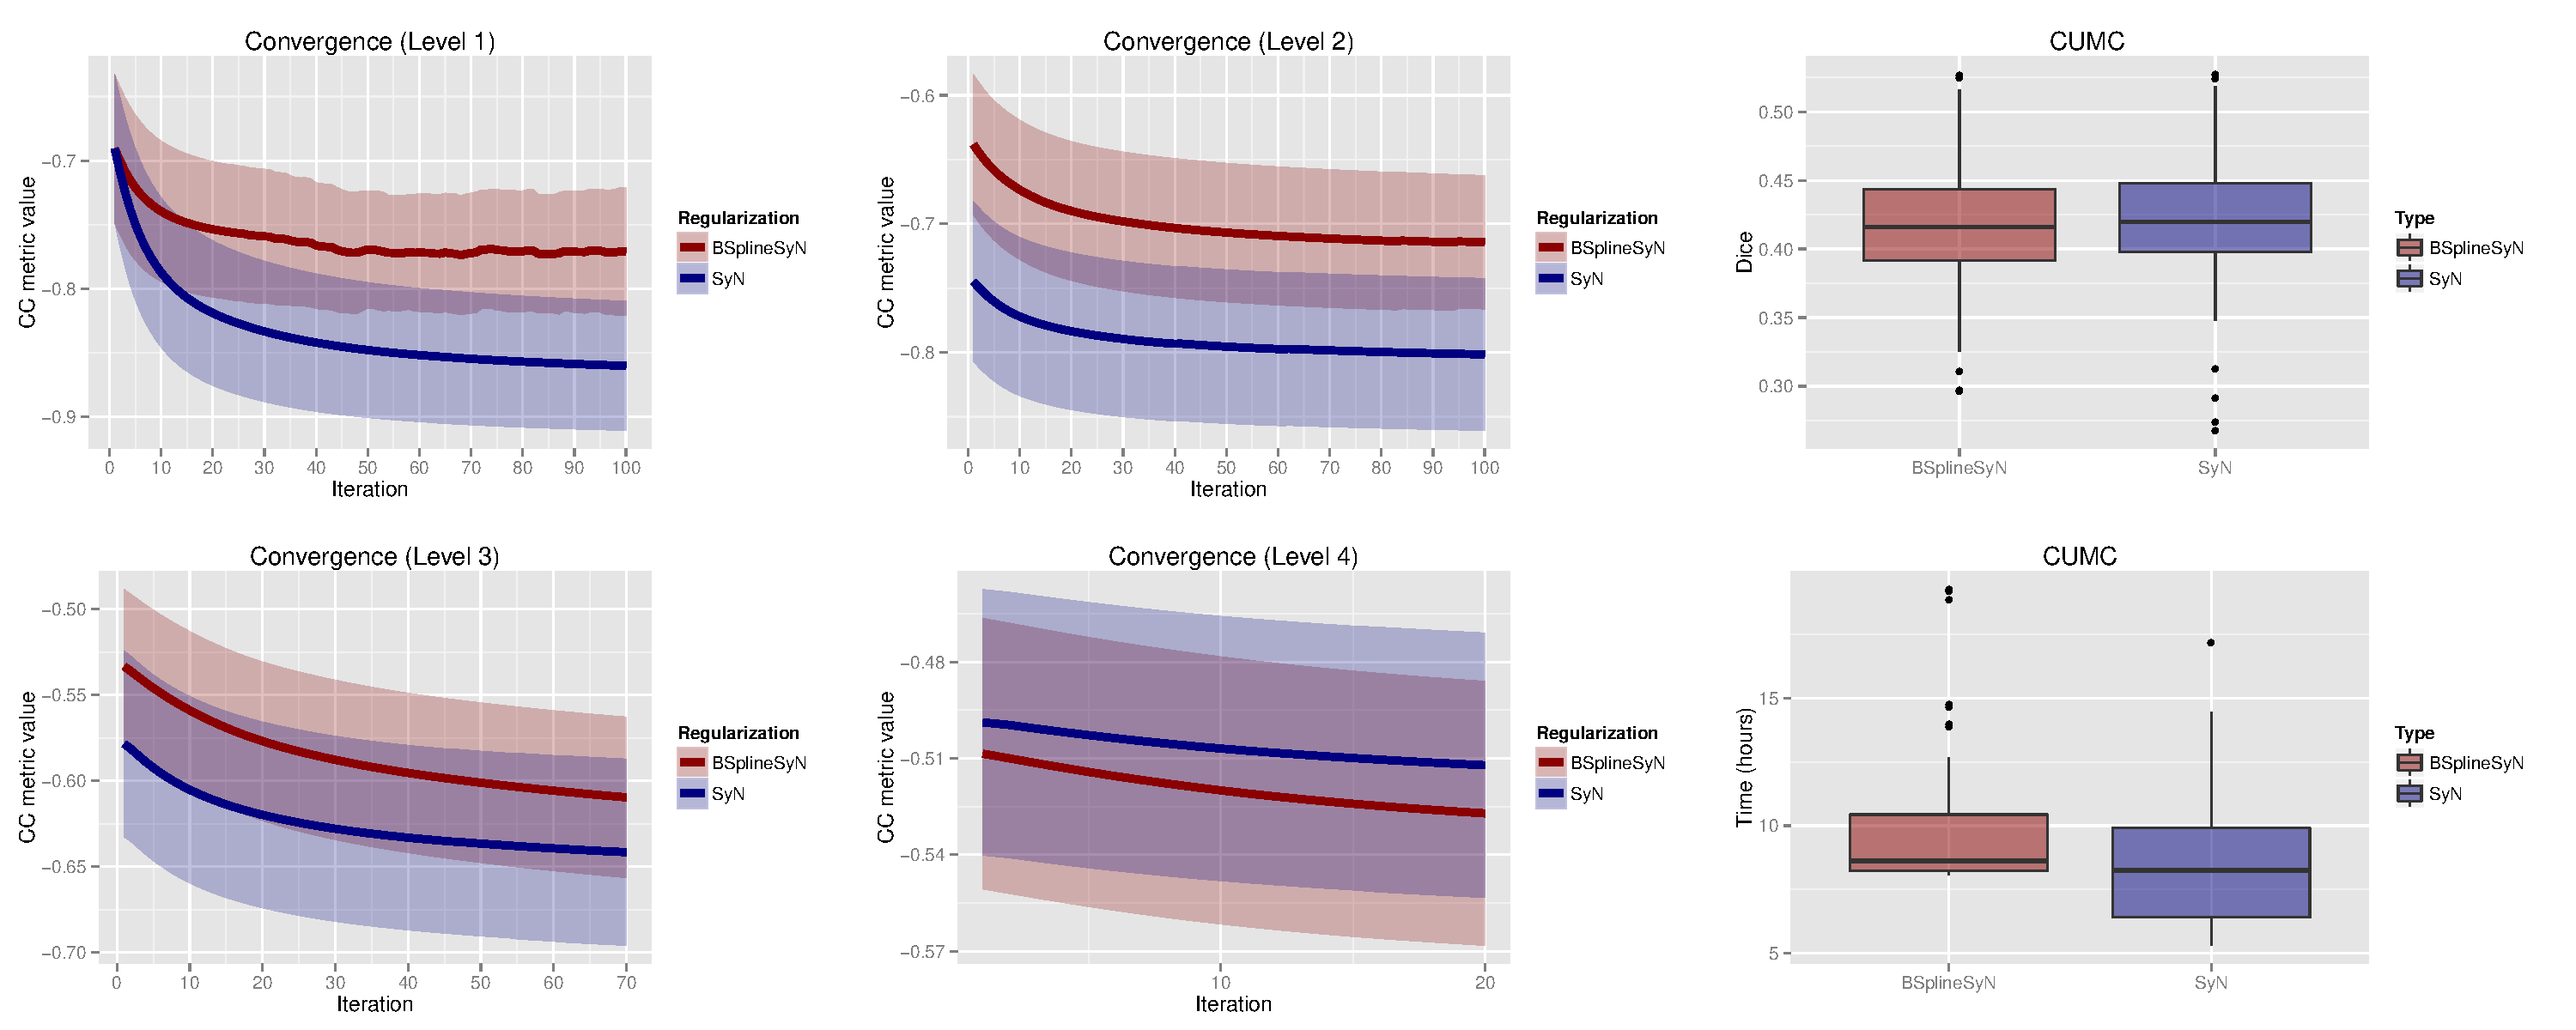
\includegraphics[width=0.95\textwidth]{allCUMC.pdf}
  \caption{}
\end{figure}

\begin{figure}[htb]
  \centering
  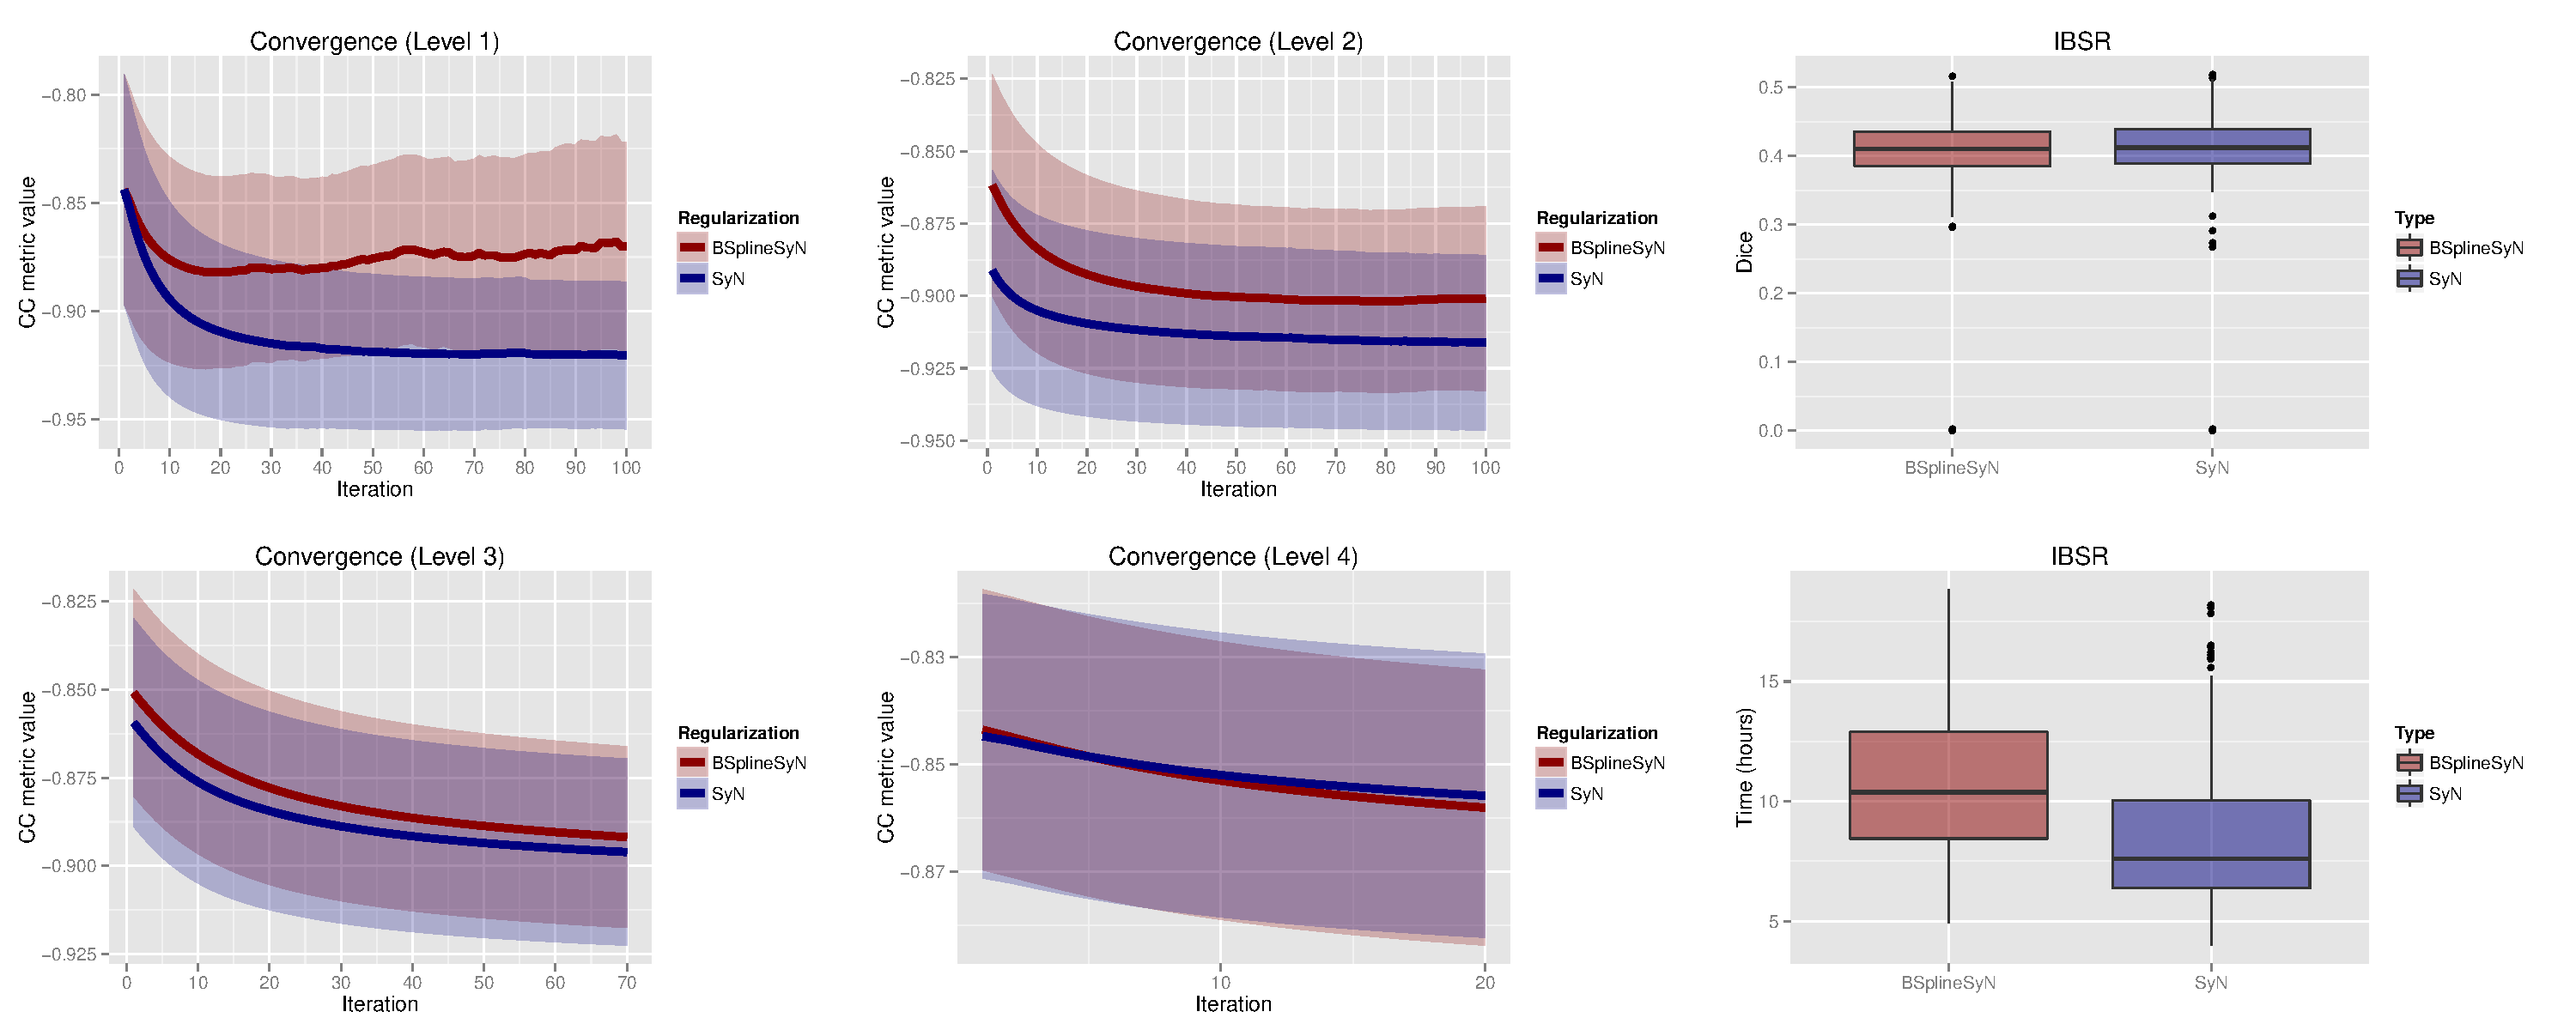
\includegraphics[width=0.95\textwidth]{allIBSR.pdf}
  \caption{Currently redoing on the cluster.}
\end{figure}

\begin{figure}[htb]
  \centering
  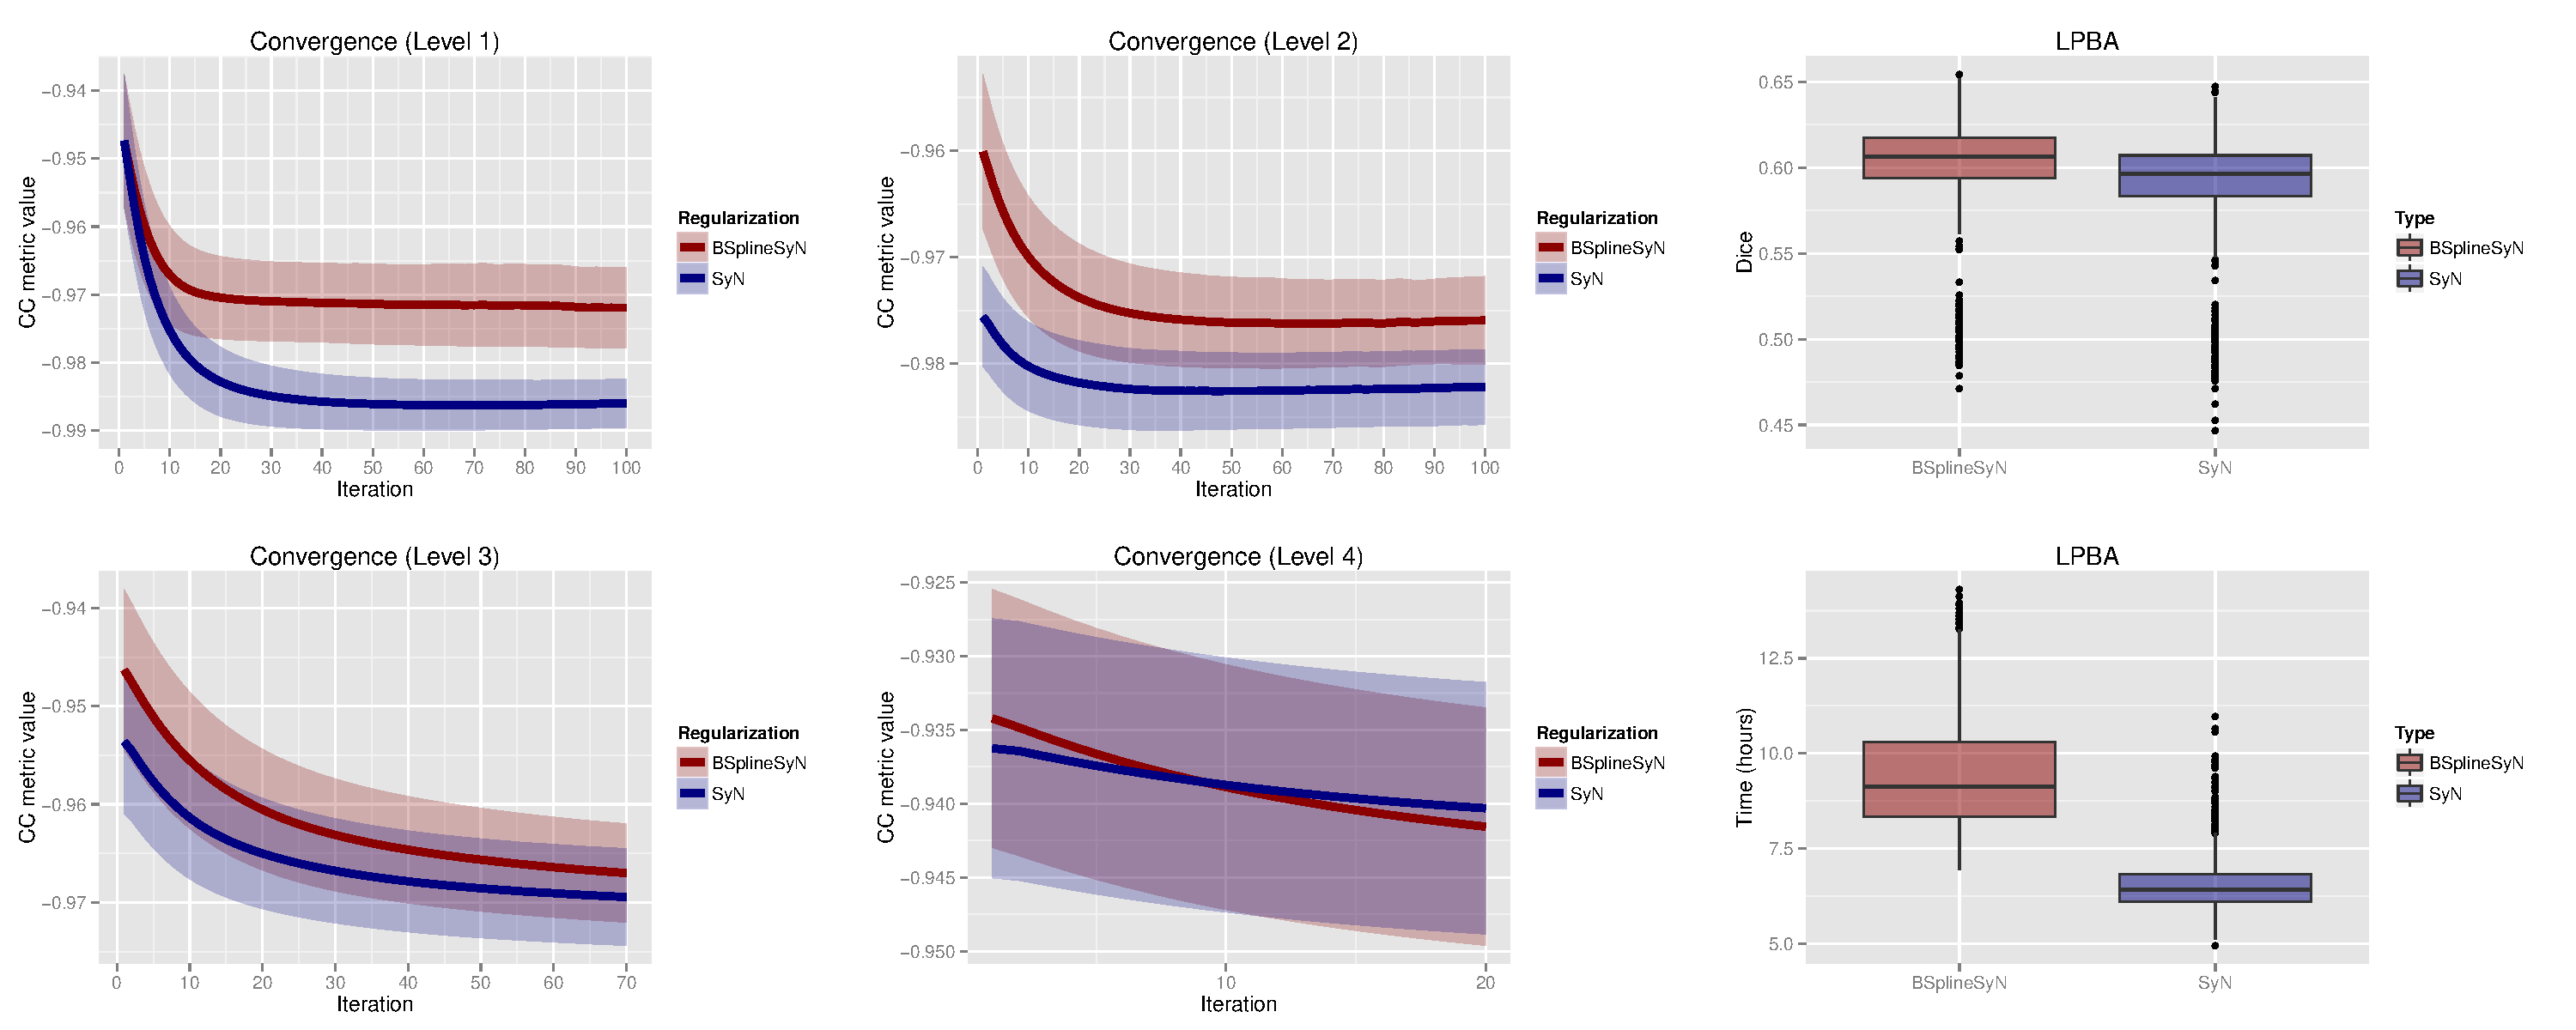
\includegraphics[width=0.95\textwidth]{allLPBA.pdf}
  \caption{}
\end{figure}

\begin{figure}[htb]
  \centering
  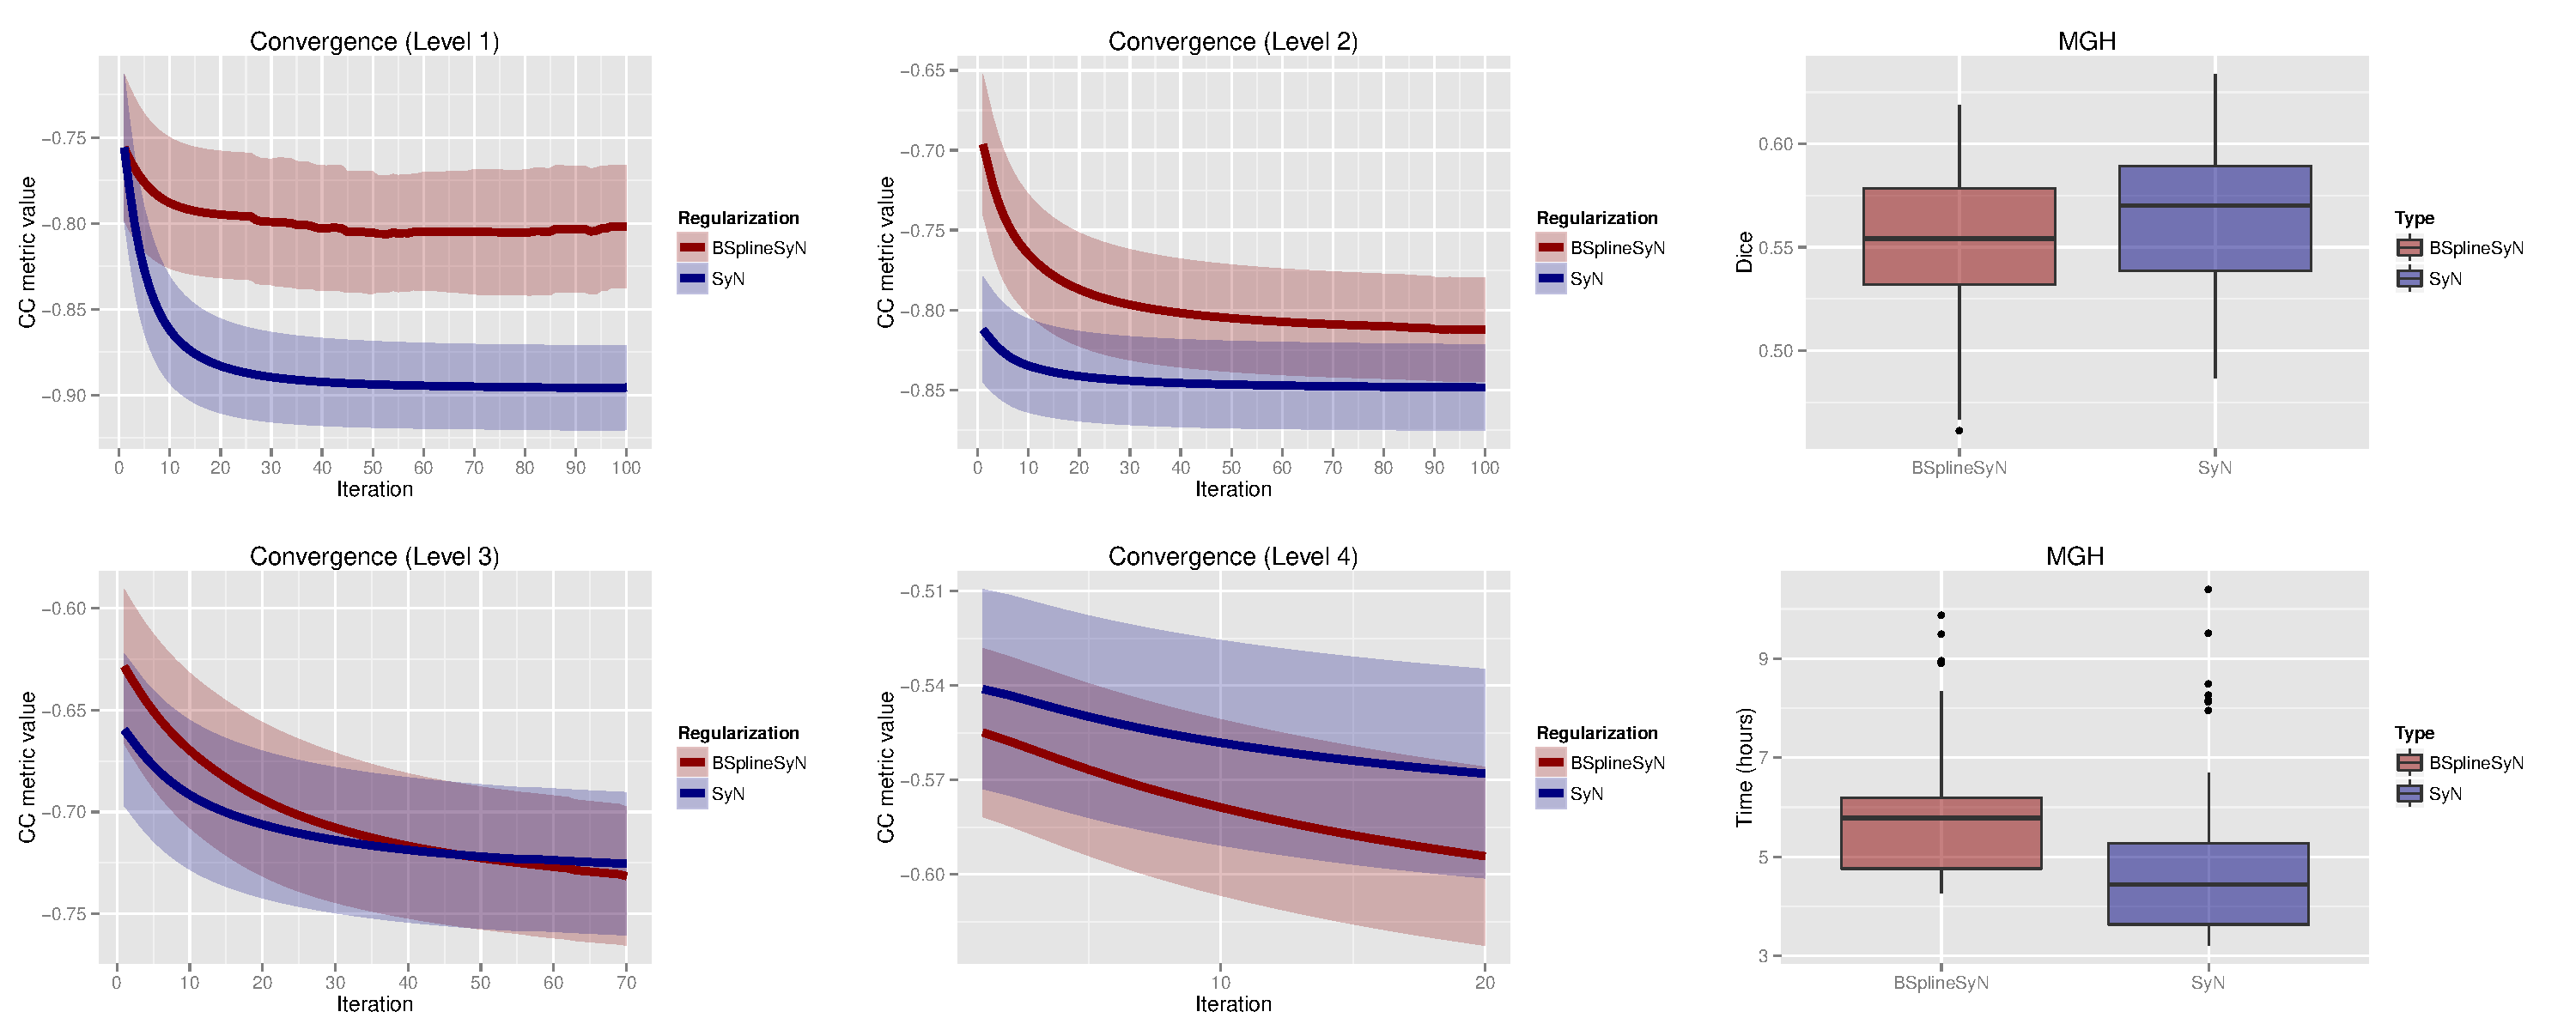
\includegraphics[width=0.95\textwidth]{allMGH.pdf}
  \caption{Currently redoing on the cluster.}
\end{figure}

\begin{figure}[htb]
  \centering
  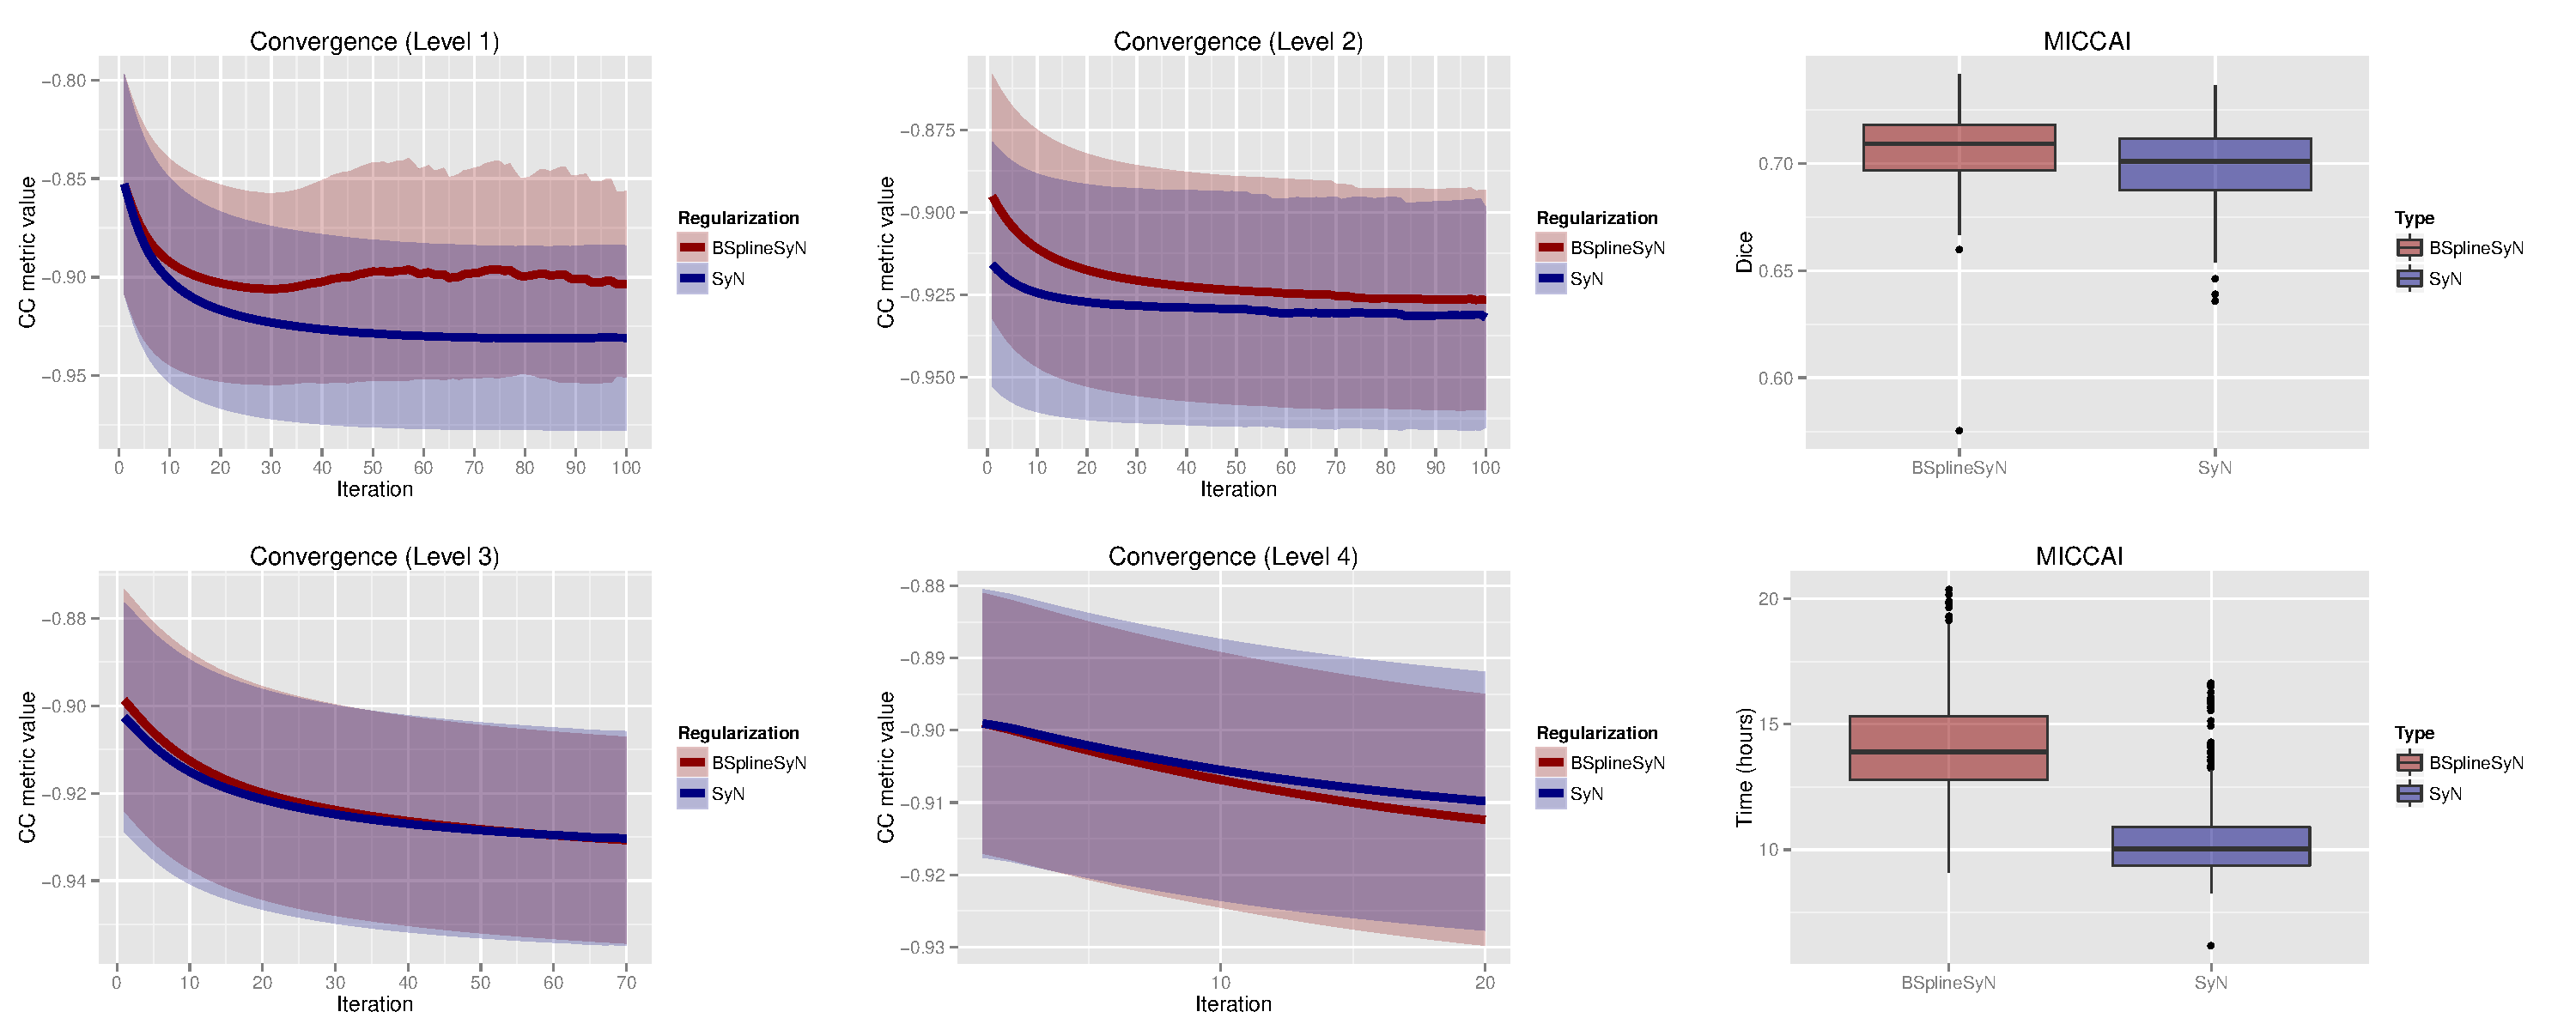
\includegraphics[width=0.95\textwidth]{allMICCAI.pdf}
  \caption{}
\end{figure}



\section{Discussion and Conclusions}
%This should explore the significance of the results of the work, not repeat them. A combined Results and Discussion section is often appropriate. Avoid extensive citations and discussion of published literature.

B-spline regularization is easily adapted into the diffeomorphic registration framework and performs comparably to analogous algorithms which we demonstrated in the case of SyN.  Even more importantly, all source code and data used in this work is publicly available for the interested researcher to explore.

%\section{Conclusions}
%The main conclusions of the study may be presented in a short Conclusions section, which may stand alone or form a subsection of a Discussion or Results and Discussion section.

%% The Appendices part is started with the command \appendix;
%% appendix sections are then done as normal sections
%% \appendix

%% \section{}
%% \label{}

%% References
%%
%% Following citation commands can be used in the body text:
%% Usage of \cite is as follows:
%%   \citep{key}          ==>>  [#]
%%   \cite[chap. 2]{key} ==>>  [#, chap. 2]
%%   \citet{key}         ==>>  Author [#]

%% References with bibTeX database:

\bibliographystyle{frontiersinSCNS}
%\bibliographystyle{plain}
\bibliography{references}


%% Authors are advised to submit their bibtex database files. They are
%% requested to list a bibtex style file in the manuscript if they do
%% not want to use model1-num-names.bst.

%% References without bibTeX database:

% \begin{thebibliography}{00}

%% \bibitem must have the following form:
%%   \bibitem{key}...
%%

% \bibitem{}

% \end{thebibliography}


\end{document}

%%
%% End of file `elsarticle-template-1-num.tex'.
